% Part II: inference on chains (sections 4-6)
\addcontentsline{toc}{part}{Part II \quad Inference on chains}
\section{Noise, scores, and Tweedie's formula}\label{sec:noise}

\subsection{The noising channel}

All noise in this project enters through one channel. A clean value $a$ (standardised to variance one) is
replaced by
\begin{equation}\label{eq:channel}
  x=\alpha\,a+\sqrt{\Delta}\,z,\qquad \alpha=e^{-t},\quad \Delta=1-e^{-2t},\quad z\sim\N(0,1)\ \text{independent}.
\end{equation}
The \emph{noise level} $t\ge0$ runs from clean ($t=0$, $x=a$) to pure noise ($t\to\infty$, $x\approx z$). The
choice $\alpha^2+\Delta=1$ keeps the variance at one, so the channel is called \emph{variance preserving}. The
signal-to-noise ratio is $\alpha^2/\Delta=1/(e^{2t}-1)$. For a sequence, each site receives its own independent
$z_i$. The experiments use a fixed schedule of twelve levels from $t=0.05$ to $t=3$. (The consolidated note
writes $Y=X+\sigma Z$; dividing \eqref{eq:channel} by $\alpha$ shows that $\sigma=\sqrt\Delta/\alpha$.)

Equation \eqref{eq:channel} is not arbitrary: it is the exact solution at time $t$ of the Ornstein--Uhlenbeck
process started at $a$, the random motion that is pulled back towards zero while being kicked by noise. We
derive this in \S\ref{sec:langevin}; here we only need the formula.

\subsection{The score}

The density of the noised data is the clean density smoothed by the channel,
\[
  p_t(x)=\int p(a)\,\N(x;\alpha a,\Delta)\dd a,
\]
and its \emph{score} is the gradient of its logarithm,
\[
  s_t(x)=\nabla_x\log p_t(x),
\]
a vector at every point $x$ that points towards higher probability. For a Gaussian $\N(0,\Sigma)$ the score
is $-\Sigma^{-1}x$, a linear pull towards the centre.

Why the score? A diffusion generative model creates data by running the noising backwards: start from
pure noise and undo the channel step by step. The backwards dynamics has drift $x+2s_t(x)$ (a classical
result on time-reversed diffusions), so a generator needs the score at every level $t$. Knowing the score
is also knowing the density up to a constant.

\begin{caution}
Two different objects are called ``score''. The \emph{data score} $\nabla_x\log p_t(x)$ differentiates with
respect to the data; it drives denoising and generation. The \emph{parameter score}
$\partial_\theta\log p_\theta(x)$ differentiates with respect to a model parameter; it defines Fisher
information (\S\ref{sec:fisher}). Always say which variable you differentiate.
\end{caution}

\subsection{Tweedie's formula: the score is a denoiser}\label{sec:tweedie}

\begin{proposition}[Tweedie]
For the channel \eqref{eq:channel},
\begin{equation}\label{eq:tweedie}
  \nabla_x\log p_t(x)=\frac{\alpha\,\E[a\mid x]-x}{\Delta}.
\end{equation}
\end{proposition}
\begin{proof}
Differentiate $p_t(x)$ under the integral sign, using
$\nabla_x\N(x;\alpha a,\Delta)=\N(x;\alpha a,\Delta)\,(\alpha a-x)/\Delta$:
\[
  \nabla_xp_t(x)=\int p(a)\N(x;\alpha a,\Delta)\frac{\alpha a-x}{\Delta}\dd a
  =p_t(x)\,\frac{\alpha\,\E[a\mid x]-x}{\Delta},
\]
because $p(a)\N(x;\alpha a,\Delta)/p_t(x)=p(a\mid x)$ by Bayes' rule. Divide by $p_t(x)$.
\end{proof}

\begin{keyidea}
Estimating the score of noised data and computing the best denoiser $\E[a\mid x]$ are the same problem. For a
sequence, $\E[a_i\mid x_1,\dots,x_L]$ depends on \emph{every} observation, and for a non-Gaussian chain
$p_t(x_1,\dots,x_L)$ has no formula: it is an $L$-dimensional integral. The chain structure is what makes
that integral computable exactly (\S\ref{sec:bp}), in a cost that grows linearly with $L$.
\end{keyidea}

\subsection{How errors are measured}

An estimate $\hat s$ of the score is scored by its \emph{relative error} pooled over the twelve levels,
\[
  \Big(\sum_t\sum\|\hat s-s\|^2\Big/\sum_t\sum\|s\|^2\Big)^{1/2},
\]
where the inner sums run over test sequences and sites. Two reference points recur. The \emph{isotropic map} $\hat s=-x$ pretends the clean data were
independent standard Gaussians; it ignores all structure and scores about $0.67$. The \emph{linear floor} is
the score of the covariance twin (\S\ref{sec:mmse}), the best any linear method can do; at the AR(1)
laboratory with Laplace innovations it scores $0.168$, at the $\phi^4$ base cell $0.269$.

\paragraph{Check yourself.}
\begin{enumerate}[label=\thesection.\arabic*,leftmargin=2.2em]
\item Use Tweedie's formula to compute the score when $a\sim\N(0,1)$. Is the answer what you expect for the law of $x$?
\item At which noise level $t$ is the signal-to-noise ratio $\alpha^2/\Delta$ equal to one?
\end{enumerate}

\section{The Kalman filter and smoother}\label{sec:kalman}

\subsection{The model}

Take the Gaussian AR(1) chain \eqref{eq:ar1} with $q=1-\rho^2$ and observe every site through the channel:
\begin{equation}\label{eq:ssm}
  a_{i+1}=\rho a_i+\varepsilon_i,\quad\varepsilon_i\sim\N(0,q);\qquad x_i=\alpha a_i+\sqrt\Delta\,z_i .
\end{equation}
This is a \emph{linear Gaussian state-space model}: a hidden state evolving linearly with Gaussian kicks, seen
through linear Gaussian measurements. Every conditional law in it is Gaussian, so every computation reduces
to updating a mean and a variance. Two questions are natural. \emph{Filtering}: what do we know about $a_i$
from the observations up to $i$? \emph{Smoothing}: what do we know about $a_i$ from all of them?

\subsection{Filtering: predict, then update}

Suppose that after seeing $x_1,\dots,x_{i-1}$ we believe $a_i\sim\N(m_i^-,P_i^-)$ (the ``prior'' for site $i$;
for $i=1$ it is the stationary $\N(0,1)$). Two steps advance the belief.

\textbf{Update} with $x_i$: this is exactly \S\ref{sec:gausscond}. With gain $k_i=\alpha P_i^-/(\alpha^2P_i^-+\Delta)$,
\begin{equation}\label{eq:kfupdate}
  m_i=m_i^-+k_i\,(x_i-\alpha m_i^-),\qquad P_i=(1-k_i\alpha)P_i^- .
\end{equation}
\textbf{Predict} site $i+1$: push the belief through the dynamics. A Gaussian times $\rho$ plus an independent
Gaussian is Gaussian, so
\begin{equation}\label{eq:kfpredict}
  m_{i+1}^-=\rho\,m_i,\qquad P_{i+1}^-=\rho^2P_i+q .
\end{equation}
That is the whole Kalman filter: alternate \eqref{eq:kfupdate} and \eqref{eq:kfpredict}. The gain $k_i$ balances
two sources of information. If the prediction is sharp ($P_i^-$ small) the gain is small and a surprising
measurement moves the belief little; if the measurement is clean ($\Delta$ small) the gain approaches $1/\alpha$
and the belief jumps to $x_i/\alpha$. After a few sites the variances settle to a fixed point, because the
recursion for $P$ forgets its start.

\subsection{Smoothing: the Rauch--Tung--Striebel pass}

The filter at site $i$ has not used $x_{i+1},\dots,x_L$. A second, backward pass adds them.

\begin{proposition}[RTS smoother]
Let $m_i^s,P_i^s$ be the mean and variance of $a_i$ given all observations. Starting from $m_L^s=m_L$,
$P_L^s=P_L$ and going backwards,
\begin{equation}\label{eq:rts}
  m_i^s=m_i+J_i\,(m_{i+1}^s-m_{i+1}^-),\qquad P_i^s=P_i+J_i^2\,(P_{i+1}^s-P_{i+1}^-),\qquad J_i=\frac{\rho P_i}{P_{i+1}^-}.
\end{equation}
\end{proposition}
\begin{proof}
Given $x_1,\dots,x_i$, the pair $(a_i,a_{i+1})$ is Gaussian with $\Var a_i=P_i$, $\Var a_{i+1}=P_{i+1}^-$ and
$\Cov(a_i,a_{i+1})=\rho P_i$. By \eqref{eq:condmvn},
$\E[a_i\mid a_{i+1},x_{1:i}]=m_i+J_i(a_{i+1}-m_{i+1}^-)$. By the Markov property, once $a_{i+1}$ is known the later
observations say nothing more about $a_i$, so this is also $\E[a_i\mid a_{i+1},x_{1:L}]$. Averaging over $a_{i+1}$
given everything gives the mean in \eqref{eq:rts}. The variance follows from the law of total variance:
$\Var(a_i\mid x_{1:L})=(P_i-J_i^2P^-_{i+1})+J_i^2P^s_{i+1}$.
\end{proof}

Figure~\ref{fig:kalman} shows both passes on one sequence. The filter lags and is noisy, because it only
looks backwards; the smoother is smoother and tighter, because each site borrows from both sides.

\begin{figure}[h]\centering
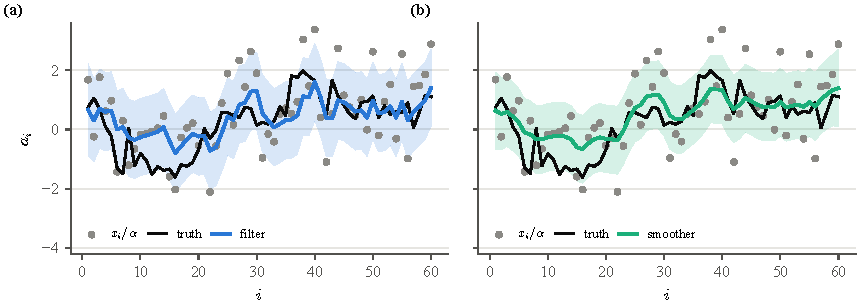
\includegraphics{primer-kalman.pdf}
\caption{A Gaussian AR(1) chain ($\rho=0.85$, black) seen through the channel at $t=0.47$ (grey dots, rescaled
by $1/\alpha$). (a) The Kalman filter mean with a two-standard-deviation band. (b) The RTS smoother: tighter, and
centred on the truth rather than lagging behind it.}
\label{fig:kalman}
\end{figure}

\subsection{What the smoother computes, and what it does not}

Everything in \eqref{eq:ssm} is jointly Gaussian, so the conditional mean is linear in the data and equals the
LMMSE estimator. Since $\Cov(a,x)=\alpha\Sigma_0$ and $\Var(x)=\alpha^2\Sigma_0+\Delta I$ with $\Sigma_0$ the clean
covariance ($\rho^{|i-j|}$),
\begin{equation}\label{eq:lmmse}
  m^s=\alpha\,\Sigma_0\big(\alpha^2\Sigma_0+\Delta I\big)^{-1}x .
\end{equation}
The smoother computes this $L$-dimensional linear solve in $O(L)$ operations instead of $O(L^3)$, by exploiting
the tridiagonal precision of the chain. Tweedie's formula \eqref{eq:tweedie} turns it into the score, and the
result is the score of the Gaussian law of $x$ itself, as it must be:
\[
  \frac{\alpha m^s-x}{\Delta}=\frac{\alpha^2\Sigma_0(\alpha^2\Sigma_0+\Delta I)^{-1}-I}{\Delta}\,x
  =\frac{\big(\alpha^2\Sigma_0-(\alpha^2\Sigma_0+\Delta I)\big)(\alpha^2\Sigma_0+\Delta I)^{-1}}{\Delta}\,x=-(\alpha^2\Sigma_0+\Delta I)^{-1}x .
\]

Now run the same recursions on a \emph{non-Gaussian} AR(1) chain, for instance with Laplace innovations of
variance $q$. The prediction step \eqref{eq:kfpredict} is still correct for the mean and variance, because the
first two moments of $\rho a+\varepsilon$ depend on $\varepsilon$ only through its mean and variance. What is lost is
everything else about the belief: its shape. Running Kalman on a non-Gaussian chain is running it on the
chain's covariance twin, and it returns \eqref{eq:lmmse} again.

\begin{inproject}
The paper's Proposition~1 makes this exact: \emph{moment-projected} belief propagation (replace every message
by the Gaussian with its mean and variance after each step, also called Gaussian closure or assumed-density
filtering) returns exactly the LMMSE estimator of the covariance twin, whatever the innovation law. So
``Gaussian closure'' and ``the linear floor'' are the same arm. On the $\phi^4$ field the projected recursion
is not even well-posed (\S\ref{sec:closurefail}), and the closure arm is the floor by definition.
\end{inproject}

\begin{caution}
The forward pass alone is the Kalman \emph{filter}; the full forward--backward computation is a
\emph{smoother}. The consolidated note asks that the two never be confused in the paper.
\end{caution}

\paragraph{Check yourself.}
\begin{enumerate}[label=\thesection.\arabic*,leftmargin=2.2em]
\item Take $P^-=1$ and the level where $\alpha^2=\Delta=\tfrac12$. Compute the gain $k$ and the filtered variance $P$.
\item Why can the smoothed variance $P_i^s$ never exceed the filtered variance $P_i$?
\end{enumerate}

\section{Hidden Markov models, Markov random fields, and belief propagation}\label{sec:bp}

\subsection{Forward and backward messages}

A \emph{hidden Markov model} is any chain \eqref{eq:chain} whose states are seen only through noisy
observations $x_i$ with likelihood $\ell_i(a)=p(x_i\mid a_i=a)$; for our channel $\ell_i(a)=\N(x_i;\alpha a,\Delta)$.
The states can be discrete (weather: sunny or rainy) or continuous (our chains). We want $p(a_i\mid x_{1:L})$
for every $i$ without integrating over all $L$ states at once. Define the forward and backward messages
\begin{equation}\label{eq:msgdef}
  \fwd_i(a)=p(x_1,\dots,x_i,\ a_i=a),\qquad \bwd_i(a)=p(x_{i+1},\dots,x_L\mid a_i=a).
\end{equation}
Splitting the sequence at site $i$ and using the Markov property,
\begin{equation}\label{eq:posterior}
  p(a_i=a\mid x_{1:L})=\frac{\fwd_i(a)\,\bwd_i(a)}{p(x_{1:L})}.
\end{equation}
Both messages obey one-step recursions. To get $\fwd_{i+1}$, sum over the value of $a_i$ (the intermediate
state), move one step with $K$, and multiply by the new likelihood:
\begin{equation}\label{eq:fwd}
  \fwd_1(a)=\mu(a)\ell_1(a),\qquad \fwd_{i+1}(a')=\ell_{i+1}(a')\int K(a'\mid a)\,\fwd_i(a)\dd a .
\end{equation}
Symmetrically, starting from $\bwd_L\equiv1$,
\begin{equation}\label{eq:bwd}
  \bwd_i(a)=\int K(a'\mid a)\,\ell_{i+1}(a')\,\bwd_{i+1}(a')\dd a' .
\end{equation}
The integrals are the matrix products \eqref{eq:matprod} on the grid: the cost is $L$ multiplications of an
$N_g$-vector by an $N_g\times N_g$ matrix, $O(LN_g^2)$, instead of the $N_g^L$ terms of brute-force summation. In
practice each message is rescaled after every step and the logarithms of the scales are accumulated, which
keeps everything in range and gives the \emph{evidence} for free:
$p(x_{1:L})=\int\fwd_L(a)\dd a$.

\begin{example}[three days of umbrellas]
A two-state chain: each day is rainy (R) or sunny (S), the weather stays the same with probability $0.8$, and
day one is R or S with probability $\tfrac12$. We never see the weather, only whether a colleague carries an
umbrella: with probability $0.9$ on a rainy day and $0.2$ on a sunny one. Over three days we see umbrella,
umbrella, no umbrella. The recursions \eqref{eq:fwd}--\eqref{eq:bwd} with sums in place of integrals give:
\begin{center}\small
\begin{tabular}{@{}lccc@{}}
\toprule
 & day 1 & day 2 & day 3 \\
\midrule
forward $(\fwd(\mathrm R),\fwd(\mathrm S))$ & $(0.450,\ 0.100)$ & $(0.342,\ 0.034)$ & $(0.0280,\ 0.0765)$ \\
backward $(\bwd(\mathrm R),\bwd(\mathrm S))$ & $(0.199,\ 0.149)$ & $(0.240,\ 0.660)$ & $(1,\ 1)$ \\
filtered $P(\mathrm R\mid\text{data so far})$ & $0.818$ & $0.910$ & $0.268$ \\
smoothed $P(\mathrm R\mid\text{all data})$ & $0.858$ & $0.785$ & $0.268$ \\
\bottomrule
\end{tabular}
\end{center}
For instance $\fwd_2(\mathrm R)=0.9\times(0.8\times0.450+0.2\times0.100)=0.342$. At every day the product
$\fwd(\mathrm R)\bwd(\mathrm R)+\fwd(\mathrm S)\bwd(\mathrm S)$ equals the same number, $0.1045$: the evidence, the probability of the
three observations. Day two shows what smoothing adds: knowing only the past, rain is $91\,\%$ likely; the dry
third day lowers it to $79\,\%$. The future revises the past, and that is the backward message's job.
\end{example}

\begin{figure}[h]\centering
\begin{tikzpicture}[node distance=1.55cm,
  hid/.style={circle,draw,thick,minimum size=0.8cm,inner sep=0pt},
  obs/.style={rectangle,draw,fill=black!8,minimum size=0.7cm,inner sep=0pt},
  >={Stealth[length=2mm]}]
\foreach \i in {1,...,5} {
  \node[hid] (a\i) at (1.9*\i,0) {$a_{\i}$};
  \node[obs] (x\i) at (1.9*\i,-1.35) {$x_{\i}$};
  \draw[->] (a\i) -- (x\i);
}
\foreach \i/\j in {1/2,2/3,3/4,4/5} { \draw[->,thick] (a\i) -- node[above,font=\scriptsize]{$K$} (a\j); }
\draw[->,very thick,keyc] (2.3,0.75) -- node[above,font=\small]{$\fwd$} (5.2,0.75);
\draw[->,very thick,warnc] (9.2,0.75) -- node[above,font=\small]{$\bwd$} (6.3,0.75);
\node[font=\scriptsize,anchor=west] at (10.0,-0.67) {$\ell_i(a)=p(x_i\mid a_i{=}a)$};
\end{tikzpicture}
\caption{A hidden Markov chain. Forward messages carry the evidence from the left, backward messages the
evidence from the right; at each site their product is the posterior \eqref{eq:posterior}.}
\label{fig:chaingraph}
\end{figure}

\paragraph{Pair marginals.} Learning (\S\ref{sec:em}) needs the posterior of \emph{neighbouring pairs},
which the same messages give:
\begin{equation}\label{eq:pair}
  \xi_i(a,a')=p(a_i=a,a_{i+1}=a'\mid x_{1:L})=\frac{\fwd_i(a)\,K(a'\mid a)\,\ell_{i+1}(a')\,\bwd_{i+1}(a')}{p(x_{1:L})}.
\end{equation}

\paragraph{Continuous states on a grid.} Replace every integral by the weighted sum \eqref{eq:trapezoid}. The
result is \emph{exact} belief propagation for the discretised model, and the discretisation error is measured,
not assumed: on Gaussian chains the grid reproduces the closed-form smoother \eqref{eq:rts} to double
precision, and against a four-times finer grid the score changes by less than $10^{-5}$ relative on ordinary
data. When the chain is Gaussian, every message in \eqref{eq:fwd}--\eqref{eq:bwd} is a Gaussian bump and the
recursions reduce to the Kalman filter and smoother: grid BP carries $401$ numbers where $2$ would do, which is
why it is a diagnostic there and a necessity elsewhere.

\subsection{Markov random fields: the undirected view}

The same chain can be written without arrows. A \emph{Markov random field} on a graph assigns to every
configuration an energy built from local terms and sets
\begin{equation}\label{eq:mrf}
  p(a)=\frac{1}{\Zp}\exp\big(-\En(a)\big),\qquad \En(a)=\sum_{\text{edges }(i,j)}W(a_i,a_j)+\sum_iU(a_i),
\end{equation}
with $\Zp=\int e^{-\En}$ the \emph{partition function}. The pair energy $W$ rewards compatible neighbours, the
site energy $U$ favours some values. The defining property is local: given its neighbours, a site is
independent of everything else, because only the terms touching it change when it changes. (The
Hammersley--Clifford theorem says that for positive densities this local property and the factorisation
\eqref{eq:mrf} are equivalent.) A \emph{hidden} Markov random field adds noisy observations of each site;
since the likelihood is a product of site terms, the posterior is again a Markov random field with $U$
replaced by $U-\log\ell_i$. Denoising is inference in a hidden Markov random field.

On a two-dimensional grid (images) the graph has loops and exact inference is hopeless; one uses
approximations such as Besag's iterated conditional modes, Gibbs sampling (Geman and Geman) or loopy belief
propagation. On a line there are no loops, and everything is exact.

\paragraph{Transfer matrices.} On a chain, write $T(a,a')=e^{-W(a,a')-U(a)/2-U(a')/2}$ (splitting each site term
between its two bonds). Then the partition function is a product of matrices,
\[
  \Zp=\int\!\!\cdots\!\!\int T(a_1,a_2)T(a_2,a_3)\cdots T(a_{L-1},a_L)\,(\text{boundary terms}),
\]
each integral being the sum over an intermediate index in \eqref{eq:matprod}. Belief propagation, the
forward--backward algorithm and the transfer-matrix method of statistical physics are \emph{one computation in
three languages}.

\subsection{From undirected back to directed: the hidden future factor}\label{sec:futurefactor}

A chain-shaped random field is a Markov chain, but its transition kernel is \emph{not} simply $e^{-W(a,\cdot)}$
normalised. Condition on $a_i$: the law of $a_{i+1}$ is proportional to $T(a_i,a_{i+1})$ times the total weight
of all ways the chain can continue from $a_{i+1}$ to the right end, which is a backward message of the
unobserved chain. Arriving at a value from which many good continuations exist is more likely. For a long
chain this ``future factor'' becomes the leading eigenvector of $T$ (\S\ref{sec:transfer}). Keep this in mind:
it is the origin of the tilt in the tilted walk (\S\ref{sec:synthesis}).

\subsection{Belief propagation in general}

On any graph without loops (a tree), \emph{sum-product} belief propagation passes messages along edges: the
message from a node to a neighbour is the sum, over the node's value, of its local factor times the pair
factor times all messages it received from its \emph{other} neighbours. After one sweep inwards and one
outwards every node holds its exact marginal. On a chain this is \eqref{eq:fwd}--\eqref{eq:bwd}. Replacing sums
by maximisations gives \emph{max-product} (the Viterbi algorithm), which finds the single most probable
configuration rather than the posterior mean. Drawing $a_L$ from its posterior and then $a_i$ from
$p(a_i\mid a_{i+1},x)\propto\fwd_i(a_i)K(a_{i+1}\mid a_i)$ going leftwards samples whole configurations from the
posterior (forward filtering, backward sampling).

\subsection{When Gaussian closure breaks}\label{sec:closurefail}

Gaussian closure replaces each message by a Gaussian with its mean and variance. For a message that says ``the
next site is in one of two wells, $+1$ or $-1$'', the Gaussian with the same moments is a broad bump centred at
zero, on the barrier, where the field almost never is. On the $\phi^4$ chain something stronger happens: from
any value far outside the bulk, the kernel jumps straight back into the bulk, so the backward message
$\bwd_i(a)$ is nearly flat over the whole grid and its moment projection is meaningless. Measured: $38$--$43\,\%$ of
a projected message's mass sits in the outer $5\,\%$ of the grid at the base cell and $98$--$100\,\%$ on the other
cells (E32, E33 oracles). This is why the closure arm of the field experiments is the linear floor.

\paragraph{Check yourself.}
\begin{enumerate}[label=\thesection.\arabic*,leftmargin=2.2em]
\item Brute force would sum over every configuration of the hidden chain. For $L=32$ sites on a grid of $N_g=401$
  points, compare the number of terms with the cost of belief propagation.
\item In the umbrella example, recompute $\bwd_2(\mathrm R)$ from \eqref{eq:bwd} and check that
  $\fwd_2(\mathrm R)\bwd_2(\mathrm R)+\fwd_2(\mathrm S)\bwd_2(\mathrm S)$ is the evidence.
\end{enumerate}
